\section{Unified Modeling Language (UML)}

\hspace{1cm} The Unified Modeling Language (UML) is a graphical language for 
visualizing, specifying, constructing, and documenting software-intensive systems. 
This language is maintained by the Object Management Group (OMG) \cite{UML}.

UML is one of the most widely used modeling languages for describing real-world 
application domains. It works with various object and component methods to represent 
software systems. As software systems grow in size, complexity, and distribution, 
building and maintaining them becomes more challenging. UML helps reduce this 
complexity by providing a high level of abstraction that captures essential 
information needed for designing and developing software systems.

UML includes multiple diagram types, each focusing on different aspects of a design. 
These diagrams fall into two main categories: (1) structural diagrams that represent 
the static aspects of a system, and (2) behavioral diagrams that describe the dynamic 
aspects. These structural and behavioral categories collectively contain fourteen 
different diagram types, as specified in the UML Reference Manual \cite{UML_Reference_Manual}.

For this thesis, two structural diagrams are particularly relevant:

%%% Sample
% The Unified Modeling Language (UML) is a graphical language for 
% visualizing, specifying, constructing, and documenting software-intensive systems.
% This unified language is maintained by the Object Management Group (OMG) [58].
% The UML has become one of the most widely used modeling language that can
% be used with all significant object and component methods for describing real-world
% application domains. Software systems, in today’s world, are growing in size, complex
% ity, distribution and importance. As a result, building and maintenance of software
% have become a more complex and challenging task. Therefore, the deployment of
% languages such as UML reduces the complexity and difficulty by providing a high
% level of abstraction, which describes precise and essential information for designing
% and developing the software system [50].  
% The graphical representation of the UML includes a set of diagrams, each focusing
% on different aspects of a design. The UML Notation Guide states all the notation of 
% diagram elements [58]. These diagrams can be classified into two groups (a) a structural
% diagram that represents the static aspect of the system, and (b) a behavioral diagram
% that describes the dynamic aspect of the system. Altogether, fourteen different model
% types can be found in the Unified Modeling Language Reference Manual [71]. In this
% thesis, two diagrams, i.e., class diagram and object diagram, have
% been extensively used and are explained further in this section.

\subsection{Class Diagram}
Class diagrams are the most common diagram type in object-oriented modeling. 
They illustrate the static structure of a system by depicting classes, their 
attributes, operations, and the relationships between classes. Classes 
represent sets of objects, where attributes describe the values these objects 
may contain, and operations specify the behaviors objects can perform.
Associations in class diagrams describe connections between different classes, 
with multiplicity indicators showing how many objects of one class can be linked 
to objects of another class. Class diagrams also include other relationship types: 
aggregation and composition (both representing whole-part relationships, with 
different levels of dependency), and generalization (inheritance relationship 
where specialized classes inherit properties from a general class).

% Example here
\begin{figure}
    \begin{center}
        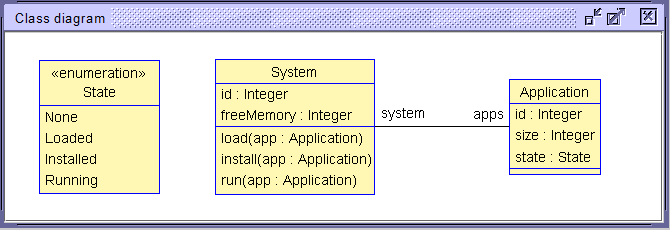
\includegraphics[width=0.8\textwidth]{figures/c1/Class_diagram.png}
        \caption{Class diagram of the Software System Model.}
        \label{fig:class_diagram_software_system_model}
    \end{center}
\end{figure}

Figure \ref{fig:class_diagram_software_system_model} shows an example class diagram
of a software system. This system has id and freeMemory attributes. The id attribute
is used to uniquely identify each instance of the software system. The freeMemory
attribute is used to store the amount of free memory available in the system. The
system also has three operations 
% TODO: Finish this paragraph

These diagrams form the foundation of object-oriented modeling and are essential 
for understanding the system structure that our temporal and event-based extensions 
will work with. In this thesis, class diagrams provide the structural framework 
upon which temporal properties will be defined and verified.

%%% Version 1
% Class diagrams show the static structure of a system by depicting classes, 
% their attributes, operations, and relationships between classes. These diagrams 
% form the foundation of object-oriented modeling and capture how objects relate 
% to one another. Class diagrams are important for understanding the system structure 
% that our temporal and event-based extensions will work with.

%%% Sample
% Class diagrams are the most common diagram found in object-oriented modeling
%  systems. It illustrates the static design view of the system model and shows classes
%  of the system, their attributes, operations and associations [64]. The classes reflect
%  a set of objects. The attributes describe values that the objects may contain, and
%  an operation specifies the result of the behavior of objects. The associations describe
%  connections among the different class objects, and they can refer to each other through
%  role names. The number of objects of one class linked to other class objects depends
%  on the multiplicity attached to an association end.
% The class diagram can also have other elements such as aggregation, composition
% and generalization to show the relationship between classes. Aggregation and compo
% sition are a whole-part relationship. In aggregation, the relationship between a child
% class and parent class is independent, whereas, in composition, they are dependent.
% A generalization is a relationship between classes in which one class is identified as
% the general class and the others as the specialization of it. A specialized class inherits
% all the properties and characteristics from the general class.

\subsection{Object Diagram}
Object diagrams are structural diagrams that represent real-world entities or 
modeled system elements as concrete instances of classes. While class diagrams 
show abstract structures, object diagrams provide snapshots of a system at specific 
points in time, showing actual objects with specific attribute values and the links 
connecting them [77].

Objects in these diagrams are instances of classes defined in the class diagram, 
with concrete values assigned to their attributes. Links between objects are 
instances of the associations defined in the class diagram. This concrete 
representation makes object diagrams particularly valuable for verification purposes.

% Example here
[Example here]

An important limitation of object diagrams is that they represent only a single 
state of the system. When the system state changes through operation calls, 
previous state information is lost. A single object diagram cannot represent 
the flow of information or system evolution over time. This limitation is 
particularly relevant to our work, as it highlights why standard UML/OCL approaches 
struggle with temporal specifications. In this thesis, object diagrams play a crucial 
role in our validation approach, where sequences of object diagrams (filmstrips) 
are used to represent and verify temporal properties.

%%% Version 1
% Object diagrams provide snapshots of a system at specific points in time, showing 
% actual instances of classes (objects) and their relationships. While class diagrams 
% show abstract structures, object diagrams show concrete system states with specific 
% values. These diagrams are useful for verification purposes as they show examples 
% of system configurations that meet or violate constraints. In this thesis, object 
% diagrams play an important role in validating temporal properties through the 
% filmstrip approach.

%%% Sample
% Object diagrams are also a type of structural diagram. It represents the entitites of the
%  real world, or of the modeled system, as instances of the classes described in the class
%  diagram, and their relationships as links, which are instances of the corresponding
%  associations. Objects are defined by concrete attribute values and a link connects
%  the objects participating in the association. In general, an object diagram provides
%  a snapshot of a system at a particular point in time showing objects, their attribute
%  values, and links connecting the objects [77].
% The object diagram represents only the single state of a class diagram. So, the
%  previous state information can be lost due to the change in the system state through
%  the operation call. Therefore, a single object diagram cannot represent any flow of
%  information of a state.